\subsection{Echo State Networks}

Jaeger proposed the \textit{Echo State Network} \cite{jaeger_echo_2001} as an
alternative approach to RNNs, in which only the weights of the output units are
modified. In RNNs, the activation state $\mathbf{x}(t)$ is determined as a
function of the sequence of inputs that is fed to the network $\mathbf{u}(t),
\mathbf{u}(t-1), \ldots$ making its activation an ``echo'' of the input history.
% (TODO): only in some cases does it have the "echo" state property^.

\begin{figure}[H]
  \centering
  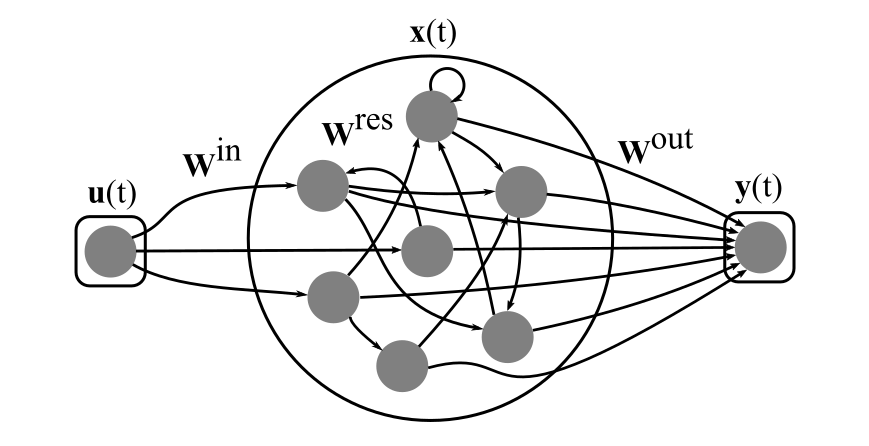
\includegraphics[width=2.5in]{img/esn.png}
  \caption{
    Basic architecture of ESN reservoir systems. The reservoir acts as a
high-dimensional kernel, transforming the temporal input sequence into a spatial
representation. The readout is trained with supervision, providing a least
squares optimum.
  }
  \label{esn}
\end{figure}
% (TODO): Figure lacks labels for weights and such; what's what^?

In this paper, we consider discrete-time RNNs with $N$ internal network nodes, a
single input, and a single output node. Fig. \ref{esn} illustrates the basic
architecture of such ESN reservoirs. The reservoir state is updated according to

\begin{equation}
  \mathbf{x}(t + 1) =
    \tanh(\mathbf{W}^{res}\mathbf{x}(t)
        + \mathbf{W}^{in}\mathbf{u}(t)),
  \label{xt}
\end{equation}

\noindent using $\tanh$ as the nonlinear transfer function for internal
reservoir nodes. The output of the reservoir is given by

\begin{equation}
  \mathbf{y}(t + 1) =
    \mathbf{W}^{out}\mathbf{x}(t).
  \label{yt}
\end{equation}

To train an ESN model of size N in offline mode, it is run to completion on a
training set. The reservoir states are represented by an Nth order column vector
$\mathbf{X}$, and the one-dimensional output by a first order column vector
$\mathbf{Y}$. The linear readout layer is then trained to minimize the squared
output error $E = \norm{\mathbf{Y} - \mathbf{\hat{Y}}}$ where
$\mathbf{\hat{Y}}$ is the target output, which amounts to solving a system of
linear equations

% (TODO): We use the NRMSE. Add this^.

\begin{equation}
  \mathbf{\hat{Y}} = \mathbf{W}^{out}\mathbf{X}.
  \label{hatreg}
\end{equation}

Well-known methods of solving (\ref{hatreg}) include ridge regression, often
called Tikhonov regularization

\begin{equation}
  \mathbf{W}^{out} = \mathbf{\hat{Y}}\mathbf{X}^{T}
                    (\mathbf{X}\mathbf{X}^{T} + \lambda_{r}\mathbf{I})^{-1},
  \label{tikhonov}
\end{equation}

\noindent where $\lambda_{r}$ is a regularization coefficient, and the
Moore-Penrose pseudo-inverse

\begin{equation}
  \mathbf{W}^{out} = \mathbf{\hat{Y}}\mathbf{X}^{+}.
  \label{pseudo}
\end{equation}

When the network is adapted to $\mathbf{W}^{out}$, the ESN is fully trained,
thus illustrating the apparent simplicity and low algorithmic complexity of the
method. Gauging the performance of a trained network is done by running a test
set. We use the normalized root mean square error (NRMSE) for this evaluation,
given a predicted signal $\mathbf{y}(t)$ and a target signal
$\mathbf{\hat{y}}(t)$

\begin{equation}
  E(\mathbf{y}, \mathbf{\hat{y}}) = \sqrt{\frac{
      \mean{\norm{\mathbf{y}(t) - \mathbf{\hat{y}}(t)}^{2}}
    }{
      \mean{\norm{\mathbf{\hat{y}}(t) - \mean{\mathbf{\hat{y}}(t)}}^{2}}
    }
  }
  .
  \label{nrmse}
\end{equation}
% (TODO): The formality of these error calculations, some call it RNMSE some
% NRMSE. I use from Reservoir Computing Approaches to Recurrent Neural Network
% Training by Jaeger.

\subsection{Reservoir generation}

As with virtually every machine learning technique, the application of ESNs
requires some experience. Although a conceptually simple idea, generating
adequate reservoir networks is influenced by multiple global
parameters. Recommendations to achieve sufficient performance are presented in
\cite{montavon_practical_2012, jaeger_tutorial_nodate}, suggesting parameters
such as the scaling of the input weight matrix, the spectral radius of the
reservoir connection matrix, the leaking rate of reservoir nodes, and the model
size parameters of high importance. However, in practice the evaluation of a
reservoir is an endeavor often conducted by training the output and measuring
the error, sometimes requiring extensive parameter sweeps.

% (TODO): Talk more about specific parameters^?

% (TODO): Write about how Wres and Win are created etc. What _we_ do can be
% discussed in Method. Cite good explanatory articles on this.

% (TODO): Change this to matrix notation: Y filled with y and X filled with
% x. Must be done multiple places.

\subsection{Assessing the quality of a reservoir}

This is not quite easy. CHARC? Why we chose NARMA, since it's fairly simple.

% (TODO): See part V. of Comparative Study of Reservoir Computing for Temporal
% Signal Processing.

\subsection{NARMA}

Nonlinear autoregressive moving average (NARMA) \cite{atiya_new_2000} is a class
of time series models widely used to benchmark the performance of recurrent
neural networks. We use the NARMA10 task to evaluate the emulation performance
of an ESN, which is a temporal task with a time-lag of ten time steps given by

% (TODO): Cite any NARMA users? Many listed in Kubota 2019^.

\begin{equation}
  y_{t+1} = \alpha y_{t} +
  \beta y_{t} \sum_{i=0}^{9}y_{t-i} +
  \gamma u_{t}u_{t-9} +
  \delta,
  \label{narma}
\end{equation}

\noindent with the default constant parameters set to $\alpha = 0.3$, $\beta =
0.05$, $\gamma = 1.5$ and $\delta = 0.1$. The input $u_{t}$ is an i.i.d. stream
drawn from the interval [0, 0.5]. The task presents a challenge of both memory
and nonlinearity, uncovered to be a universal trade-off in in dynamical systems
\cite{dambre_information_2012, verstraeten_memory_2010}, making it a well-suited
task. The dynamical anatomy of the NARMA10 task was further investigated in
\cite{kubota_dynamical_2019}.

% (TODO): How many time steps? Minimum complexity cites this. Should we scale
% input?

% END

% 1. How ESNs work. Why ESNs are chosen to approximate physical systems; what can
% it tell us about such physical limitations? Cite practical guide to ESNs by Luko
% and Adaptive Nonlinear System Identification. Ridge regression, pseudo inverse,
% how it's done.

% 2. Time series, specifically NARMA and NARMA 10. Also write about practical
% applications of RC range. Why are ESNs not useless? Some example applications in
% Verstraeten's thesis and Reservoir Computing Trends by Jaeger. Achieves great
% performance in temporal processing tasks. Also relate this to Dambre paper on
% the fundamental information processing capabilities, it's a fundamental
% question.

% Introduce the problem statements individually for each limitation. ''Natural
% computational systems must have specific topologies, and the uniform random
% connectivity is not appropriate.'' Topology discussion, Manevitz et. al.

%%% Local Variables:
%%% mode: latex
%%% TeX-master: "../main"
%%% End:
